\documentclass[11pt, a4paper]{article}

% --- ΡΥΘΜΙΣΕΙΣ ΓΛΩΣΣΑΣ & ΓΡΑΜΜΑΤΟΣΕΙΡΩΝ (LuaLaTeX) ---
\usepackage{fontspec}
\usepackage[english, greek]{babel} % Ελληνικά ως προεπιλογή

% Ορισμός γραμματοσειρών με fallback
\setmainfont{FreeSerif}[
    BoldFont = FreeSerifBold,
    ItalicFont = FreeSerifItalic
]
\setsansfont{FreeSans}
\setmonofont{FreeMono}

% --- ΠΑΚΕΤΑ ΜΟΡΦΟΠΟΙΗΣΗΣ ---
\usepackage[a4paper, top=2.5cm, bottom=2.5cm, left=2.5cm, right=2.5cm]{geometry}
\usepackage{titlesec}
\usepackage{parskip}
\usepackage{hyperref}
\usepackage{graphicx}
\usepackage{xcolor}
\usepackage{listings}
\usepackage{enumitem}
\usepackage{fancyhdr}
\usepackage{amsmath}
\usepackage{float} % Απαραίτητο για το [H] placement
\usepackage{booktabs} % Για επαγγελματικούς πίνακες

% Ορισμός χρωμάτων για επαγγελματική εμφάνιση
\definecolor{darkblue}{rgb}{0.0, 0.2, 0.4}
\definecolor{gray}{rgb}{0.5, 0.5, 0.5}

% --- ΚΕΦΑΛΙΔΕΣ / ΥΠΟΣΕΛΙΔΑ ---
\pagestyle{fancy}
\fancyhf{}
\rhead{JazzMate Report}
\lhead{Ιωάννης Μπουρίτης}
\cfoot{\thepage}

\begin{document}

% --- ΠΡΟΣΑΡΜΟΣΜΕΝΗ ΠΡΩΤΗ ΣΕΛΙΔΑ ---
\begin{titlepage}
    \centering
    \vspace*{0.5cm}
    
    % Πανεπιστημιακό Ίδρυμα
    {\large \textsf{Πολυτεχνείο Κρήτης}} \\
    {\small \textsf{Σχολή Ηλεκτρονικών Μηχανικών και Μηχανικών Υπολογιστών}} \\
    \vspace{1.5cm}
    
    % Λογότυπο (Αν έχεις αρχείο εικόνας, αφαίρεσε το σχόλιο παρακάτω)
    % \includegraphics[width=0.3\textwidth]{tuc_logo.png} 
    \vspace{1cm}
    
    % Οριζόντια γραμμή
    \rule{\linewidth}{0.8mm} \\[0.6cm]
    
    % Τίτλος Έργου
    {\Huge \bfseries \textcolor{darkblue}{JazzMate}} \\[0.4cm]
    {\Large \textit{Ανάπτυξη Πράκτορα Ενισχυτικής Μάθησης για \\ Διαδραστικό Μουσικό Αυτοσχεδιασμό}} \\[0.6cm]
    
    \rule{\linewidth}{0.8mm} \\
    \vspace{1.5cm}
    
    % Μάθημα
    {\large \textbf{Αυτόνομοι Πράκτορες}} \\
    \vspace{2.5cm}
    \textbf{Ιωάννης Μπουρίτης} \\
            2021030173
    
    \vfill
    
    % Ημερομηνία
    {\large Χειμερινό Εξάμηνο \\ \today}
    
\end{titlepage}

\newpage
\thispagestyle{empty}
\tableofcontents
\newpage

% ---------------------------------------------------------------------

\section{Εισαγωγή και Στόχος}
Η παρούσα εργασία πραγματεύεται την ανάπτυξη του \textbf{JazzMate}, ενός αυτόνομου πράκτορα (autonomous agent) ικανού να παράγει Jazz αυτοσχεδιασμούς (solo) σε πραγματικό χρόνο. Στόχος ήταν η δημιουργία ενός συστήματος που δεν βασίζεται σε άκαμπτους κανόνες (hard-coded rules), αλλά μαθαίνει να "αισθάνεται" τη μουσική μέσω \textbf{Ενισχυτικής Μάθησης (Reinforcement Learning - RL)}.

Ο πράκτορας καλείται να αντιμετωπίσει ένα δυναμικό περιβάλλον όπου η αρμονία (συγχορδίες) αλλάζει συνεχώς και πρέπει να επιλέξει τις κατάλληλες νότες, παύσεις και διάρκειες ώστε το αποτέλεσμα να είναι μουσικά ευχάριστο και δημιουργικό.

\section{Αρχιτεκτονική Συστήματος}

\subsection{Αλγόριθμος και Εργαλεία}
Για την εκπαίδευση του πράκτορα επιλέχθηκε ο αλγόριθμος \textbf{Deep Q-Network (DQN)}, με χρήση της πολιτικής \texttt{MultiInputPolicy} από τη βιβλιοθήκη \textit{Stable-Baselines3}. Ο αλγόριθμος εκπαιδεύτηκε για 200,000 βήματα (timesteps) ώστε να επιτύχει σταθερή σύγκλιση.
\begin{itemize}
    \item \textbf{Γλώσσα:} Python
    \item \textbf{Βιβλιοθήκες:} Gymnasium (Custom Environment), Stable-Baselines3 (DQN), Mido (MIDI I/O), FluidSynth (Synthesis).
\end{itemize}

\subsection{Μοντελοποίηση Προβλήματος (MDP)}
Το πρόβλημα ορίστηκε ως μια Διαδικασία Λήψης Αποφάσεων Markov:
\begin{itemize}
    \item \textbf{State (Observation Space):} Ένας συνδυασμένος χώρος (Dict) που περιέχει:
    \begin{itemize}
        \item \textbf{Chord Tones:} Διάνυσμα 12 θέσεων (Multi-hot encoding) που υποδεικνύει ποιες νότες ανήκουν στην τρέχουσα συγχορδία.
        \item \textbf{Step Progress:} Η σχετική θέση μέσα στο κομμάτι ($0 \to 1$).
        \item \textbf{Last Action \& Held Duration:} Η προηγούμενη επιλογή και η διάρκεια διατήρησής της.
        \item \textbf{Style Seed:} Έναν τυχαίο παράγοντας για την ενθάρρυνση διαφορετικών προσεγγίσεων.
    \end{itemize}
    \item \textbf{Action Space:} 38 διακριτές επιλογές:
    \begin{itemize}
        \item 0-35: Νότες σε εύρος 3 οκτάβων (C3 έως B5).
        \item 36: Παύση (Rest).
        \item 37: Κράτημα Νότας (Hold).
    \end{itemize}
\end{itemize}

\section{Τεχνικές Λεπτομέρειες Εκπαίδευσης}

\subsection{Υπερπαράμετροι Αλγορίθμου}
Η εκπαίδευση του DQN πράκτορα πραγματοποιήθηκε με τις ακόλουθες υπερπαραμέτρους:

\begin{table}[H]
\centering
\begin{tabular}{@{}ll@{}}
\toprule
\textbf{Παράμετρος} & \textbf{Τιμή} \\ \midrule
Συνολικά Timesteps & 200,000 \\
Learning Rate ($\alpha$) & $1 \times 10^{-4}$ \\
Replay Buffer Size & 50,000 transitions \\
Batch Size & 32 (default) \\
Target Network Update ($\tau$) & 1.0 (hard update) \\
Target Network Update Frequency & 10,000 steps \\
Gamma ($\gamma$) - Discount Factor & 0.99 (default) \\
Exploration Fraction & 0.4 (40\% των timesteps) \\
Initial Exploration ($\epsilon_{start}$) & 1.0 \\
Final Exploration ($\epsilon_{end}$) & 0.05 \\
\bottomrule
\end{tabular}
\caption{Υπερπαράμετροι του DQN αλγορίθμου}
\label{tab:hyperparameters}
\end{table}

\subsection{Στρατηγική Εξερεύνησης}
Χρησιμοποιήθηκε η κλασική \textbf{$\epsilon$-greedy} στρατηγική με γραμμική φθίνουσα εξερεύνηση:

\begin{equation}
\epsilon(t) = \max\left(\epsilon_{end}, \epsilon_{start} - \frac{t}{T_{explore}} \cdot (\epsilon_{start} - \epsilon_{end})\right)
\end{equation}

όπου $T_{explore} = 0.4 \times 200000 = 80000$ timesteps.

Αυτό σημαίνει ότι:
\begin{itemize}
    \item \textbf{Timesteps 0--80,000:} Το $\epsilon$ μειώνεται γραμμικά από 1.0 σε 0.05, επιτρέποντας στον πράκτορα να εξερευνά ενεργά νέες στρατηγικές.
    \item \textbf{Timesteps 80,000--200,000:} Το $\epsilon$ παραμένει σταθερό στο 0.05, δίνοντας έμφαση στην εκμετάλλευση (exploitation) της μαθημένης πολιτικής.
\end{itemize}

\subsection{Δομή Επεισοδίων}
Κάθε επεισόδιο (episode) αποτελείται από μία ολοκληρωμένη μουσική εκτέλεση:
\begin{itemize}
    \item \textbf{Μήκος Progression:} Κάθε φορά που καλείται το \texttt{reset()}, δημιουργείται μια τυχαία ακολουθία 8 συγχορδιών, με κάθε συγχορδία να διαρκεί 16 steps.
    \item \textbf{Συνολικά Steps ανά Episode:} $8 \times 16 = 128$ steps/episode.
    \item \textbf{Αριθμός Επεισοδίων:} Για 200,000 συνολικά timesteps: 
    \begin{equation}
    N_{episodes} = \frac{200000}{128} \approx 1562 \text{ επεισόδια}
    \end{equation}
\end{itemize}

Κατά την εκπαίδευση, ο πράκτορας έπαιξε συνολικά \textbf{περίπου 1562 διαφορετικά μουσικά κομμάτια}, εξερευνώντας χιλιάδες διαφορετικούς συνδυασμούς συγχορδιών.

\subsection{Experience Replay και Neural Network}
Το DQN χρησιμοποιεί:
\begin{itemize}
    \item \textbf{Replay Buffer:} Αποθηκεύονται οι τελευταίες 50,000 μεταβάσεις $(s, a, r, s', done)$.
    \item \textbf{Mini-batch Updates:} Σε κάθε βήμα εκπαίδευσης, δειγματοποιούνται τυχαία 32 transitions για gradient descent.
    \item \textbf{Target Network:} Ανανεώνεται πλήρως (hard update) κάθε 10,000 steps για σταθεροποίηση της εκπαίδευσης.
\end{itemize}

Η νευρωνική αρχιτεκτονική (\texttt{MultiInputPolicy}) χειρίζεται αυτόματα το Dict observation space, εξάγοντας χαρακτηριστικά από κάθε στοιχείο ξεχωριστά (chord tones, progress, action history) και στη συνέχεια τα συνδυάζει σε ένα κοινό latent representation.

\subsection{Μετρικές Παρακολούθησης}
Η εκπαίδευση παρακολουθήθηκε μέσω του \textbf{Monitor wrapper} του Gymnasium, το οποίο καταγράφει:
\begin{itemize}
    \item \textbf{Episode Reward ($R_{total}$):} Το άθροισμα των rewards σε κάθε επεισόδιο.
    \item \textbf{Episode Length:} Πάντα 128 steps (σταθερό μήκος επεισοδίου).
    \item \textbf{Timestep:} Ο συνολικός αριθμός βημάτων μέχρι στιγμής.
\end{itemize}

Τα δεδομένα αποθηκεύονται στο αρχείο \texttt{training\_logs/monitor.csv} και απεικονίζονται στη γραφική παράσταση της Ενότητας 4.4.

\section{Η Διαδικασία Εκπαίδευσης: Reward Shaping}

Η συνάρτηση ανταμοιβής ($R$) σχεδιάστηκε με στόχο την ισορροπία μεταξύ αρμονικής ορθότητας και μελωδικής ελευθερίας.

\subsection{Αρμονία και Μελωδική Ροή}
Ο πράκτορας λαμβάνει $+1.0$ για νότες εντός συγχορδίας και $-0.6$ για "λάθος" νότες. Ταυτόχρονα, πριμοδοτούνται τα μικρά μελωδικά διαστήματα (διαστήματα 1-2 ημιτονίων λαμβάνουν $+0.8$), ενώ τιμωρούνται αυστηρά τα μεγάλα πηδήματα (διάστημα $>9$ λαμβάνει $-1.5$), προωθώντας τη δημιουργία ομαλών μελωδικών γραμμών.

\subsection{Καταπολέμηση της Μονοτονίας (Anti-Pattern Detection)}
Ένα από τα σημαντικότερα κομμάτια του κώδικα είναι η αποτροπή των "λούπων".
\begin{itemize}
    \item \textbf{Exact Note Repeats:} Η επανάληψη της ίδιας νότας τιμωρείται άμεσα ($-2.0$ για την πρώτη επανάληψη, $-10.0$ για κάθε επόμενη).
    \item \textbf{Sequence Loops:} Εισήχθη μηχανισμός ελέγχου ιστορικού (History). Αν ο πράκτορας επαναλάβει μοτίβα 2, 3 ή 4 νοτών (π.χ. A-B-A-B), δέχεται κλιμακωτές ποινές από $-5.0$ έως $-15.0$.
\end{itemize}

\subsection{Ενθάρρυνση "Riffs" και Φρασεολογίας}
Για να μην γίνει ο πράκτορας υπερβολικά παθητικός λόγω των ποινών:
\begin{itemize}
    \item \textbf{Riff Bonus:} Μια αλληλουχία 4-5 διαφορετικών νοτών ανταμείβεται με $+2.5$ έως $+4.0$.
    \item \textbf{Musical Phrasing:} Δίνεται η μέγιστη ανταμοιβή ($+3.0$) όταν ο πράκτορας επιλέξει παύση (\textbf{Rest}) αμέσως μετά από ένα πετυχημένο riff, διδάσκοντάς του να "αναπνέει" μουσικά.
\end{itemize}

\subsection{Ανάλυση Καμπύλης Εκμάθησης}
Παρακάτω παρουσιάζεται η πορεία εκπαίδευσης του πράκτορα για 200.000 βήματα.

\begin{figure}[H]
    \centering
    \framebox{\parbox{0.9\textwidth}{\centering
        \vspace{0.3cm}
        % Σιγουρέψου ότι το αρχείο training_graph.png υπάρχει στον ίδιο φάκελο
        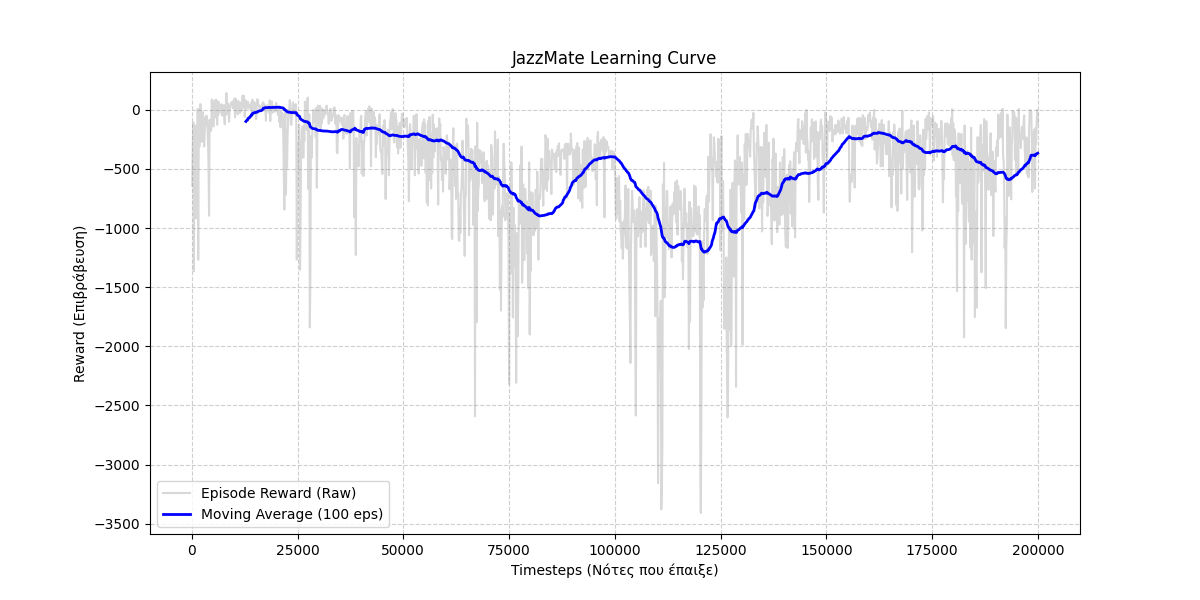
\includegraphics[width=0.95\linewidth]{../training_graph.png}
        \vspace{0.3cm}
    }}
    \caption{\textbf{Καμπύλη Εκμάθησης (Learning Curve):} Η μπλε γραμμή αναπαριστά τον κυλιόμενο μέσο όρο (moving average) της επιβράβευσης. Παρατηρούμε μια αρχική πτώση (dip) γύρω στα 100k βήματα, η οποία οφείλεται στην εισαγωγή αυστηρών ποινών και στην εξερεύνηση. Στη συνέχεια, ο πράκτορας προσαρμόζεται, μαθαίνει να αποφεύγει τις επαναλήψεις και η απόδοση ανακάμπτει σταθερά.}
    \label{fig:learning_curve}
\end{figure}

\noindent\textbf{Ερμηνεία Φάσεων Εκπαίδευσης:}
\begin{enumerate}
    \item \textbf{Αρχική Εξερεύνηση (0--50k):} Υψηλή διακύμανση λόγω τυχαίας εξερεύνησης ($\epsilon \approx 1.0 \to 0.4$). Μέσος όρος reward περίπου $-200$ έως $-400$.
    
    \item \textbf{Φάση Προσαρμογής (50k--100k):} Παρατηρείται πτώση στην απόδοση καθώς εφαρμόζονται οι ποινές anti-spam. Ο πράκτορας δοκιμάζει νέες στρατηγικές.
    
    \item \textbf{Ανάκαμψη (100k--150k):} Εμφανής βελτίωση καθώς ο πράκτορας μαθαίνει να συνδυάζει αρμονία, ποικιλία και phrasing. Το $\epsilon$ έχει πέσει στο 0.05.
    
    \item \textbf{Σταθεροποίηση (15α0k--200k):} Σύγκλιση σε σταθερή απόδοση με μέσο reward γύρω στο $-400$ έως $-600$, που αντιστοιχεί σε μουσικά αποδεκτά solos.
\end{enumerate}

\section{Διαδραστικότητα και Υλοποίηση Player}

Το σύστημα αναπαραγωγής (\texttt{play\_jazz.py}) μετατρέπει τις αποφάσεις του AI σε ζωντανή μουσική.

\subsection{Humanization και Στυλ}
Εφαρμόζεται αλγόριθμος \textbf{Swing} με αυξομείωση του χρόνου των steps (1.3x / 0.7x) και δυναμικές εντάσεις (velocity) ανάλογα με το τονικό ύψος. Ο χρήστης μπορεί να επιλέξει μεταξύ \textbf{Simple Block Chords} και \textbf{Arpeggio} για τη συνοδεία του αριστερού χεριού.

\subsection{Jam Mode}
Το σύστημα υποστηρίζει πλήρως εξωτερικούς MIDI Controllers. Μέσω ενός callback μηχανισμού, το πρόγραμμα ενημερώνεται ακαριαία για την αλλαγή συγχορδίας που προκαλεί ο χρήστης πατώντας νότες-βάσεις στο κλαβιέ, επιτρέποντας έναν διαδραστικό αυτοσχεδιασμό "ανθρώπου-μηχανής".

\section{Συμπέρασμα και Μελλοντικές Επεκτάσεις}
Το JazzMate αποδεικνύει ότι η Ενισχυτική Μάθηση μπορεί να κωδικοποιήσει σύνθετες καλλιτεχνικές έννοιες μέσω προσεκτικού Reward Shaping. Ο πράκτορας παρουσιάζει συνοχή, αποφεύγει τη στατικότητα και ανταποκρίνεται αρμονικά στις αλλαγές.

\begin{enumerate}
    \item \textbf{Ολοκληρωμένη "Ορχήστρα":} Επέκταση του συστήματος για την ταυτόχρονη παραγωγή μουσικής από πολλαπλά όργανα (π.χ. πιάνο, μπάσο και τύμπανα), δημιουργώντας ένα πλήρες αυτοσχεδιαστικό σύνολο.
    \item \textbf{Δυναμική Αναγνώριση Συγχορδιών:} Αντικατάσταση της στατικής αντιστοίχισης πλήκτρου-συγχορδίας με έναν αλγόριθμο αναγνώρισης σε πραγματικό χρόνο, επιτρέποντας στον χρήστη να παίζει ελεύθερα σύνθετες συγχορδίες τις οποίες το μοντέλο θα αναγνωρίζει αυτόματα.
    \item \textbf{Πολυπρακτορική Υλοποίηση (Multi-Agent):} Εκπαίδευση διαφορετικών πρακτόρων με διαφορετικές "μουσικές προσωπικότητες" και κανόνες. Ένα ανώτερο σύστημα αποφάσεων θα μπορεί να εναλλάσσει τους πράκτορες, αποφεύγοντας τη μονοτονία και εξασφαλίζοντας ότι το αποτέλεσμα θα ακούγεται πάντα φρέσκο.
    \item \textbf{RL από Ανθρώπινη Ανατροφοδότηση (RLHF):} Ενσωμάτωση ενός μηχανισμού όπου ο μουσικός-συνεργάτης θα βαθμολογεί την απόδοση του πράκτορα σε πραγματικό χρόνο. Αυτό θα επιτρέψει στο μοντέλο να προσαρμόζεται δυναμικά στο υποκειμενικό γούστο και το στυλ του εκάστοτε συνεργάτη.
\end{enumerate}

\end{document}